\documentclass[10pt, conference, compsocconf]{IEEEtran}
\usepackage[brazil]{babel}  % Português
 
%\usepackage{unicode} % Acentos Português, compatibilizando o Windows com o texto
\usepackage[utf8x]{inputenc} % utfx é uma gambiarra para funcionar com mais caracteres..bizarrisse do windows.
\usepackage{rotating}
\usepackage{longtable}
\usepackage{booktabs}
\usepackage{graphicx}
\usepackage{multicol}
\usepackage{amssymb}
\usepackage{multicol}
\usepackage{subfigure}
 

\begin{document}
%
% paper title 
\title{
	Identificação Precoce de Fadiga em Atletas por Reconhecimento de Padrões em Movimentos Oculares e Variabilidade da Frequência Cardíaca
}

%------------------------------------------------------------------------- 
% change the % on next lines to produce the final camera-ready version 
\newif\iffinal
%\finalfalse
\finaltrue
 
\iffinal
  \author{
    \IEEEauthorblockN{Diego Schmaedech}
     \IEEEauthorblockA{
      Laboratório de Educação Cerebral\\
      UFSC, Florianópolis, Brasil\\
      schmaedech@gmail.com}
     \and
      \IEEEauthorblockN{Prof. Dr. Emílio Takase}
      \IEEEauthorblockA{
       Laboratório de Educação Cerebral\\
      UFSC, Florianópolis, Brasil\\
      takase@educacaocerebral.com}
      \and
      \IEEEauthorblockN{Joana Bastos}
      \IEEEauthorblockA{
       Laboratório de Educação Cerebral \\
      UFSC, Florianópolis, Brasil\\
      djoubm@gmail.com}
  }
\else
    \author{Sibgrapi paper ID: 1806903277}
\fi
%------------------------------------------------------------------------- 

 

% make the title area
\maketitle
 
\begin{abstract}
	
	Na maioria dos esportes a falta de instrumentos para identificar a fadiga faz com que muitos técnicos e atletas não percebam o excesso de treinamento e acabem vivenciando a chamada Síndrome do Excesso de Treinamento (SET), que causa danos físicos e mentais, incluindo o abandono do esporte pelo atleta. 
	O objetivo deste trabalho é desenvolver e validar um protocolo para identificação precoce da fadiga em atletas utilizando instrumentos de medição de variáveis psicofisiológicas de baixo custo e métodos de reconhecimento de padrões aplicado ao conjuntos de dados multivariado das métricas extraídas de Movimentos Oculares (MO) e Variabilidade da Frequência Cardíaca (VFC). Realizando, dessa forma, uma análise da fusão dos dados de diferentes fontes.   
	
\end{abstract}


\begin{IEEEkeywords}
psicofisiologia, fadiga, reconhecimento de padrões; 

\end{IEEEkeywords}
 
\IEEEpeerreviewmaketitle

\section{Introdução}
  
	A fadiga é um processo fisiológico que pode afetar o Sistema Nervoso Central (SNC) e desencadear alterações de estados como humor e sono~\cite{Budgett1998}. O SNC ainda controla o Sistema Nervoso Autônomo (SNA), que é responsável por regular os recursos fisiológicos de acordo com as demandas do ambiente. Responder eficientemente em ambiente complexo requer um equilíbrio dinâmico entre os ramos do SNA, o sistema nervoso simpático e o sistema nervoso parassimpático~\cite{Thayer2009}. 
	
	A VFC é um importante marcador da interação entre os ramos simpáticos e parassimpáticos do SNA e tem sido estudada por ser uma medida não invasiva para identificação da fadiga. Outra medida não invasiva é variação nos movimentos oculares como piscadas e variação no diâmetro da pupila~\cite{Zhu2004}~\cite{Noor2009}.  
	 
 	Neste trabalho, será desenvolvido e validado um software de monitoramento de sinais psicofisiológicos que irá funcionar com dispositivos de baixo custo como webcams convencionais, para aquisição do MO, e frequêncimetros cardíacos comerciais (cinta toráxica), que são amplamente difundidas no meio esportivo. Este software fará parte de um protocolo para identificação de fadiga em atletas.
	%poster------------------------------------------------------------------------- 
	A fadiga é um processo fisiológico que pode afetar o Sistema Nervoso Central (SNC) e desencadear alterações de estados como humor e sono~\cite{Budgett1998}. O SNC ainda controla o Sistema Nervoso Autônomo (SNA), que é responsável por regular os recursos fisiológicos de acordo com as demandas do ambiente. Responder eficientemente em ambiente complexo requer um equilíbrio dinâmico entre os ramos do SNA, o sistema nervoso simpático e o sistema nervoso parassimpático~\cite{Thayer2009}. 
	
	A VFC é um importante marcador da interação entre os ramos simpáticos e parassimpáticos do SNA e tem sido estudada por ser uma medida não invasiva para identificação da fadiga. Outra medida não invasiva é variação nos movimentos oculares como piscadas e variação no diâmetro da pupila~\cite{Zhu2004}~\cite{Noor2009}.  
	 
 	Neste trabalho, será desenvolvido e validado um software de monitoramento de sinais psicofisiológicos que irá funcionar com dispositivos de baixo custo como webcams convencionais, para aquisição do MO, e frequêncimetros cardíacos comerciais (cinta toráxica), que são amplamente difundidas no meio esportivo. Este software fará parte de um protocolo para identificação de fadiga em atletas.
 

% make the title area  

\section{Materiais e Métodos}
	
	Participarão dessa pesquisa atletas de rendimento em diversas modalidades, eles realizarão uma bateria de tarefas antes e depois do esforço físico. Durante as tarefas cognitivas, terão sua VFC e MO monitorados e analisados. 
	 
\subsection{Participantes}

	Participarão do estudo 30 atletas de ambos os sexos em cada etapa.

\subsection{Instrumentos} 

	Na primeira etapa, serão utilizados os instrumentos: 
	
	\begin{enumerate}
\item Bateria de avaliação cognitiva computadorizada CogState: descrita em Luft~\cite{Luft2009};

\item Escala dos Estados de Humor de Brunel (BRUMS): validada também para atletas brasileiros ~\cite{Rohlfs2008};

\item Nexus-10: eletrocardiograma utilizado para monitorar a VFC com taxa amostral de 1024 Hz (montagem lead III);

\item Eyetracking: equipamento para rastreamento de olhar marca SmartEye versão 5.9 (30 Hz). 

\end{enumerate}
	   
	Na segunda etapa os dois equipamentos, Nexus-10 e Eyetracking SmartEye, serão substituídos por uma Webcam convencional com taxa de aquisição de 30 Hz e um monitor cardiofrequencímetro Polar RS 800.
	 
	 
\subsection{Processo de Coleta} 

	As coletas de dados serão realizadas individualmente. A Figura \ref{fig:processo} ilustra o processo.  
	
\begin{figure}[htb]
   \centering  
   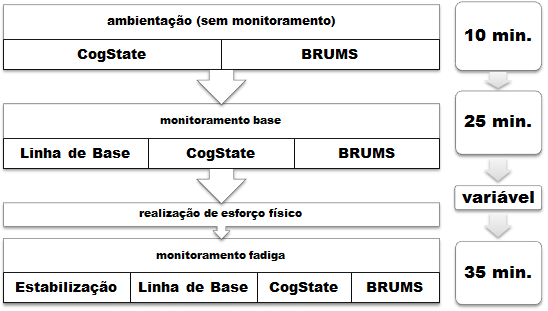
\includegraphics[scale=.6]{img/fadiga_processo}
   \caption{\it Desenho do processo realizado no protocolo. }
   \label{fig:processo}
\end{figure}

\subsection{Análise dos Dados} 

	Será realizada a validação concorrente dos dados brutos de aquisição entre os dispositivos, no caso da VFC são os dados de pulso cardíaco e no caso do MO são os dados de distância euclidiana obtida pelo processamento e análise das imagens de video. 
	
	Também serão análisadas as métricas extraídas a partir dos dados brutos, como por exemplo a Dimensão Correlacionada (D2) que é uma métrica não-linear da VFC ~\cite{Standards1996a}~\cite{Schubert2009}~\cite{Niskanen2004} e de piscadas e diâmetro da pupila~\cite{McKinley2011} que são métricas relacionadas ao MO. Para o reconhecimento de padrões serão utilizadas análises multivariadas de variância (MANOVA)~\cite{Harris01} e o algoritmo de clustering \textit{Mean Shift}~\cite{Cheng95} para classificar os níveis de SET com base nas métricas psicofisiológicas, cognitivas e dos estados de humor.
	 

\section{Discussão dos Resultados}
	 
	Até o momento foi desenvolvido o monitor de VFC, construído a partir de um microfone integrado ao frequêncimetro e o software de visão computacional que funciona a partir de webcams. Ambos funcionam em PCs convencionais. A duas interfaces de software podem ser vistas na Figura \ref{fig:softvfc}.
	
	 \begin{figure}[htb]
   \centering  
   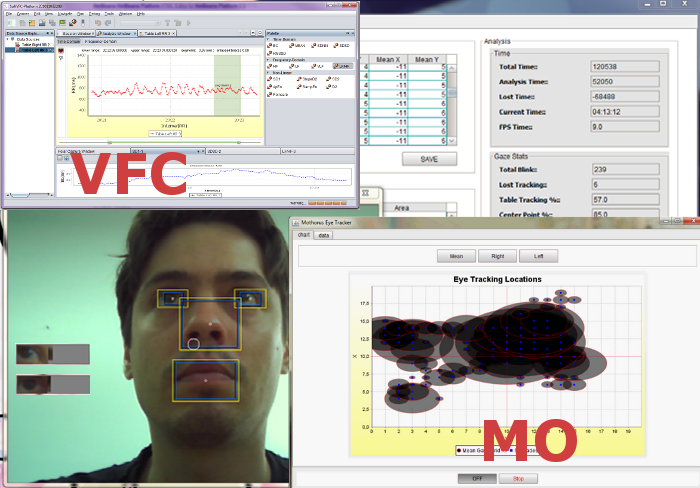
\includegraphics[scale=.5]{img/mot}
   \caption{\it Interface dos módulos desenvolvidos. }
   \label{fig:softvfc}
\end{figure}

 	O software de visão computacional foi implementado utilizando a biblioteca OpenCV~\cite{Bradski2008} e são usados os algoritmos de detecção de objetos e a técnica de \textit{template matching}, além de uma heurística própria para rastreamento. O software é capaz de detectar pequenas variações na movimentação da íris e também piscadas.
 	 
\section{Conclusão}

	A análise da VFC e MO é uma poderosa ferramenta para estudos relacionados a fadiga. Uma das contribuições deste trabalho é o desenvolvimento de um protocolo para identificação precoce de fadiga em atletas usando métodos de reconhecimento de padrões em um conjunto de dados multivariados de VFC e MO.  
	
	Este trabalho possibilitará a validação de um protocolo para a identificação precoce da fadiga de atletas, o que auxiliará os técnicos na tomada de decisão para regular as doses de treinamento, beneficiando os atletas que terão maior segurança nos treinos, podendo evitar a SET de forma mais direta. 
  
\bibliographystyle{IEEEtran}
% argument is your BibTeX string definitions and bibliography database(s)
\bibliography{ref2} 
 
\end{document}
\endinput